\documentclass{article}
\usepackage[utf8]{inputenc}
\usepackage{graphicx}
% we use paracol to display breakable two columns
\usepackage{paracol}
% define page styles using geometry
\usepackage[a4paper]{geometry}

% remove all possible margins
\geometry{top=1cm, bottom=1cm, left=1cm, right=1cm}

% indentation is zero
\setlength{\parindent}{0mm}

% include the fontawesome icon set
\usepackage{fontawesome}

\usepackage{enumitem}
\usepackage{ragged2e}
%----------------------------------------------------------------------------------------
%	FONT BASICS
%----------------------------------------------------------------------------------------

% some tex-live fonts - choose your own

\usepackage[defaultsans]{droidsans}
%\usepackage[default]{comfortaa}
%\usepackage{cmbright}
% \usepackage[default]{raleway}
%\usepackage{fetamont}
%\usepackage[default]{gillius}
%\usepackage[light,math]{iwona}
%\usepackage[thin]{roboto} 

% set font default
\renewcommand*\familydefault{\sfdefault} 	
\usepackage[T1]{fontenc}
\usepackage{moresize}
%----------------------------------------------------------------------------------------
%	TABLE /ARRAY DEFINITIONS

% extended aligning of tabular cells
\usepackage{array}

% custom column right-align with fixed width
% use like p{size} but via x{size}
\newcolumntype{x}[1]{%
>{\raggedleft\hspace{0pt}}p{#1}}%
\usepackage{xcolor}
% light color
\definecolor{darkcol}{HTML}
{A4330D}%<{type: "reference", id: "color"}>

\usepackage{fancyhdr}

\renewcommand*\headrulewidth{0pt}
\newcommand{\sidebarsection}[1]{
    \large\textcolor{darkcol}{\textbf{#1}}
}
\newcommand{\recipesection}[1]{
    \LARGE\textcolor{darkcol}{\textbf{#1}}
}
\newcommand{\preparationitem}[1]{
    \normalsize\item{#1}
}
\newcommand{\recipetext}[1]{
    \textcolor{darkcol}{#1}
}
\newcommand{\ingredientitem}[1]{
    \vspace{3pt}
    \normalsize\emph{#1}
    \vspace{3pt}
}
\begin{document}
\pagenumbering{gobble}
\columnratio{0.76}
\setlength{\columnsep}{2.2em}
\setlength{\columnseprule}{4pt}
\colseprulecolor{darkcol}
\begin{paracol}{2}
\begin{leftcolumn}

%<{type: "group", description: "Recipe information"}
\begin{center}
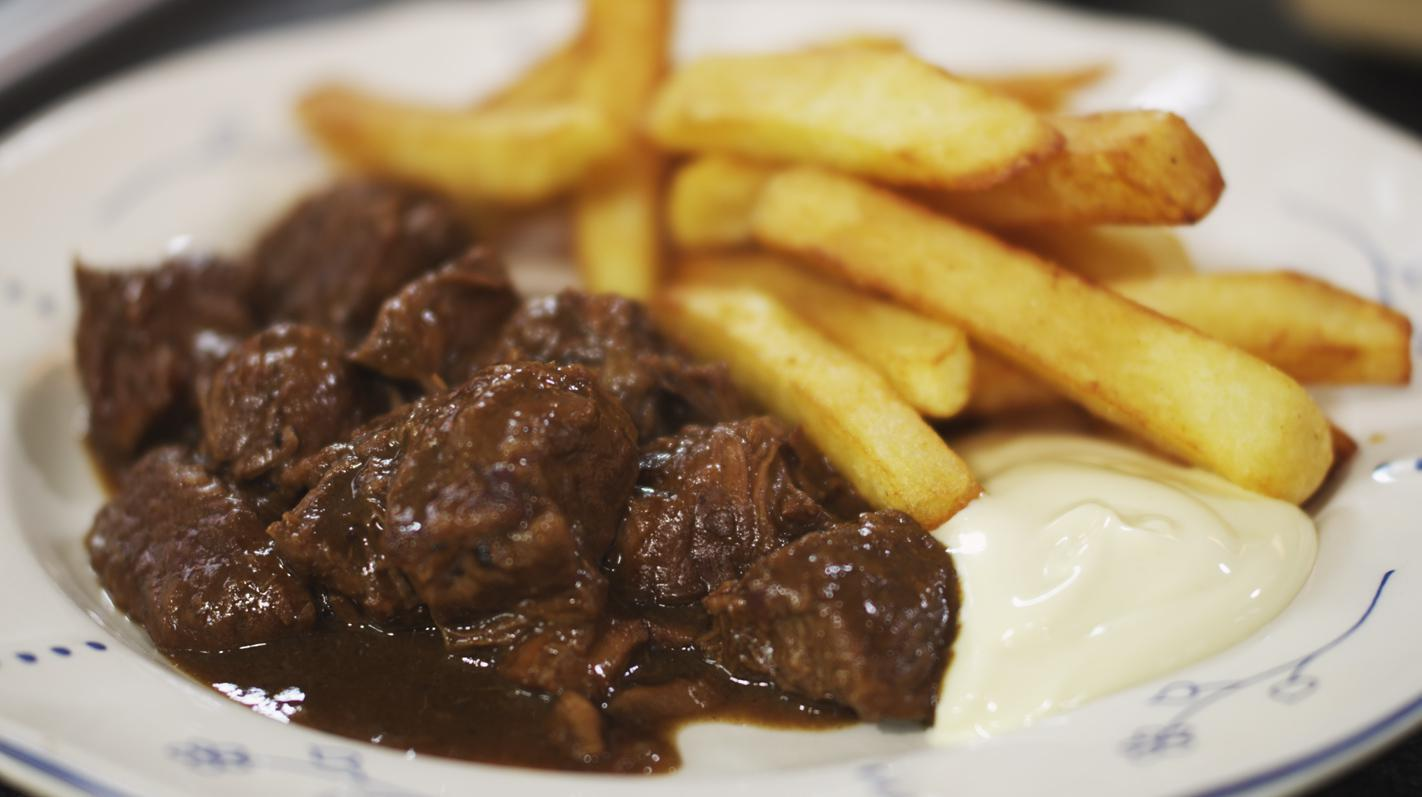
\includegraphics[width=\linewidth]{frietstoofvlees.jpg}%<{description: "Picture", type: "crop", aspect: 2, inputValue: "frietstoofvlees.jpg"}>
\end{center}
\recipesection{Recipe title} %<{description: "Recipe title", type: "text", inputValue: "Recipe title"}>
\vspace{0pt}
\\
\textcolor{darkcol}{\normalsize\faClockO\recipetext
{3 hours} %<{description: "Preparation time", type: "text", inputValue: "3 hours"}>
}
\textcolor{darkcol}{\normalsize\faUser\recipetext
{4 serves} %<{description: "Number of serves", type: "text", inputValue: "4 serves"}>
}
\textcolor{darkcol}{
\normalsize\faNewspaperO\recipetext{Some website} %<{description: "Source of recipe (optional)", type: "text", deleteOnEmpty: true, inputValue: "Some website"}>
}
%>
\vspace{5pt}
\begin{enumerate}[wide, labelwidth=!, labelindent=0pt]
    %<{description: "Preparation steps", type: "list", deleteOnEmpty: true}
        \preparationitem{Lorem ipsum dolor sit amet, consectetur adipiscing elit, sed do eiusmo.} %<{description: "Step", type: "textblock", injectBrackets: true, inputValue: "Lorem ipsum dolor sit amet, consectetur adipiscing elit, sed do eiusmo."}>
        
        \preparationitem{Lorem ipsum dolor sit amet, consectetur adipiscing elit, sed do eiusmoLorem ipsum dolor sit amet, consectetur adipiscing elit, sed do eiusmo.}
        \preparationitem{Lorem ipsum dolor sit amet, consectetur adipiscing elit, sed do eiusmo.}
        \preparationitem{Lorem ipsum dolor sit amet, consectetur adipiscing elit, sed do eiusmoLorem ipsum dolor sit amet, consectetur adipiscing elit, sed do eiusmoLorem ipsum dolor sit amet, consectetur adipiscing elit, sed do eiusmo.}
        \preparationitem{Lorem ipsum dolor sit amet, consectetur adipiscing elit, sed do eiusmoLorem ipsum dolor sit amet, consectetur adipiscing elit, sed do eiusmoLorem ipsum dolor sit amet, consectetur adipiscing elit, sed do eiusmoLorem ipsum dolor sit amet, consectetur adipiscing elit, sed do eiusmoLorem ipsum dolor sit amet, consectetur adipiscing elit, sed do eiusmo}
        \preparationitem{Lorem ipsum dolor sit amet, consectetur adipiscing elit, sed do eiusmoLorem ipsum dolor sit amet, consectetur adipiscing elit, sed do eiusmo.}
        \preparationitem{Lorem ipsum dolor sit amet, consectetur adipiscing elit, sed do eiusmo.}
        \preparationitem{Lorem ipsum dolor sit amet, consectetur adipiscing elit, sed do eiusmoLorem ipsum dolor sit amet, consectetur adipiscing elit, sed do eiusmo.}
        \preparationitem{Lorem ipsu sed do eiusmoLorem ipsum dolor siteiusmoLorem ipsum dolor sit amet, consectetur adipiscing elit, sed do eiusmoLorem ipsum dolor sit amet, consectetur adipiscing elit, sed do eiusmo.}
        \preparationitem{ipsum dolor sit amet, consectetur adipiscing elit, sed do eiusmoLorem ipsum dolor sit amet, consectetur adipiscing elit, sed do eiusmoLorem ipsum dolor sit amet, consectetur adipiscing elit, sed do eiusmoLorem ipsum dolor sit}
        \preparationitem{Lorem ipsum dolor sit amet, consectetur adipiscing elit, sed do eiusmoLorem ipsum dolor sit amet, consectetur adipiscing elit, sed do eiusmoLorem ipsum dolor sit amet, consectetur adipiscing elit, sed do eiusmo}
        \preparationitem{Lorem ipsum dolor sit amet, consectetur adipiscing elit, sed do eiusmoLorem ipsum dolor sit r sit amet, consectetur adipiscing elit, sed do eiusmo}
        \preparationitem{Lorem ipsum dolor sit amet, consectetur adipiscing elit, sed do eiusmoLorem ipsum dolor sit amet, consectetur adipiscing elit, sed do eiusmoLorem ipsum dolor sit amet, consectetur adipiscing elit, sed do eiusmoLorem ipsum doltur adipiscing elit, sed do eiusmo.}
        \preparationitem{Lorem ipsum dolor sit amet, consectetur adipiscing elit, sed do eiusmo!}
    %>

\end{enumerate}
\end{leftcolumn}

\begin{rightcolumn}

\sidebarsection{Ingredients} \\ \\
%<{description: "Ingredient list", type: "list", deleteOnEmpty: true}
\ingredientitem{2 big onions}\\ %<{description: "Ingredient", type: "text", inputValue: "2 big onions"}>
\ingredientitem{butter}\\ %<{description: "Ingredient", type: "text", inputValue: "butter"}>
\ingredientitem{1kg beef}\\ %<{description: "Ingredient", type: "text", inputValue: "1kg beef"}>
\ingredientitem{pepper and salt}\\ %<{description: "Ingredient", type: "text", inputValue: "pepper and salt"}>
\ingredientitem{2 bottles of brown beer}\\ %<{description: "Ingredient", type: "text", inputValue: "2 bottles of brown beer"}>
\ingredientitem{2 branches tyme}\\ %<{description: "Ingredient", type: "text", inputValue: "2 branches tyme"}>
\ingredientitem{2 table spoons of syrup}\\ %<{description: "Ingredient", type: "text", inputValue: "2 table spoons of syrup"}>
\ingredientitem{2 table spoons of mustard}\\ %<{description: "Ingredient", type: "text", inputValue: "2 table spoons of mustard"}>
\ingredientitem{natural vinegar}\\ %<{description: "Ingredient", type: "text", inputValue: "natural vinegar"}>
\ingredientitem{1kg (loosely cooked) potatoes for the fries}\\ %<{description: "Ingredient", type: "text", inputValue: "1kg (loosely cooked) potatoes for the fries"}>
\ingredientitem{mayonaise}\\ %<{description: "Ingredient", type: "text", inputValue: "mayonaise"}>
%>

\newcommand{\hide}[1]
{}

\hide{
    %<{type: "color", description: "Accent color (optional)", initialColor: "A4330D", id: "color", inputValue: "A4330D"}>
}

\end{rightcolumn}
\clearpage
\end{paracol}
\end{document}
